%!TEX root = ../bare_adv.tex
\subsection{Maximum Speed}
\label{sec:speed}
When an object is outside the range of sensors it is said to be vacant.
When an object is in a vacant time interval its position can be narrowed down to the cell it is located in. 
further it can be narrowed down based on the maximum speed of the object denoted $V_{max}\cdot\Delta t_1$ . 
The speed of an object type may vary, e.g. a human have a maximum recorded speed of 37.58 km/h~\cite{bolt}.
We view the range of the sensor $P_1$ as a circle with the sensors maximum range as radius, we denote this $R_1$, see Figure \ref{fig:speed1}.
Knowing the maximum speed of the object a circle can be drawn from the point where the object left the vicinity of the sensor, see $R_4$.
By drawing a circle with the radius $R_1 + R_4$, see $R_5$, is the area where the object is located. 
The next reading of a sensor of the object can be used to create a oval between the two sensor readings, see Figure \ref{fig:speed2}.  

\begin{figure}%
\centering
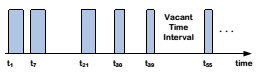
\includegraphics[width=\columnwidth]{images/vacant.png}%
\caption{The x-axis show the timestamps where the object enters the vicinity of a sensor. The colored areas are the time interval where the object in within the range of the sensor. The figure is take from~\cite{Jensen:2009:GMB:1590953.1591000}.}%
\label{fig:vacant}%
\end{figure}

\begin{figure}%
\centering
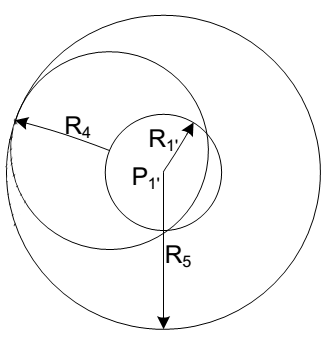
\includegraphics[width=0.5\columnwidth]{images/speed.png}%
\caption{The area that the object can move with in $V_{max}*\Delta t_1$. The figure is adapted from~\cite{Jensen:2009:GMB:1590953.1591000}.}%
\label{fig:speed1}%
\end{figure}

\begin{figure}%
\centering
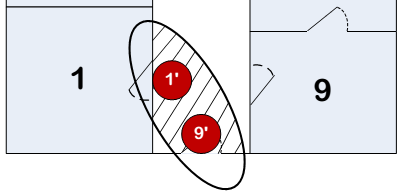
\includegraphics[width=0.8\columnwidth]{images/speed2.png}%
\caption{This figure illustrates the area where the object can be located in the vacant time between the two sensor reading. The figure is take from~\cite{Jensen:2009:GMB:1590953.1591000}.}%
\label{fig:speed2}%
\end{figure}





